\documentclass[a4paper,11pt]{article}

\usepackage[english]{babel}
\usepackage[utf8]{inputenc}
\usepackage{graphicx}
\usepackage{caption}
\usepackage{subcaption}
\usepackage[T1]{fontenc}
\usepackage{setspace}
\usepackage{geometry}
\usepackage{titling}
\usepackage{float}
\usepackage{comment}
\usepackage[backend=biber]{biblatex}
\addbibresource{refs.bib}
\usepackage{lipsum}
\usepackage{tabularx,booktabs}
\newcolumntype{C}{>{\centering\arraybackslash}X} % centered version of "X" type
\setlength{\extrarowheight}{1pt}
\usepackage[compact]{titlesec}
\titlespacing*{\title}{0pt}{*1}{*1}
%\usepackage{savetrees}
 \geometry{
 a4paper,
 total={170mm,257mm},
 left=20mm,
 top=20mm,
 right=20mm,
 bottom=20mm,
 }
\title{\normalsize\textbf{Fault Tolerance Capabilities of Three, Four and Six Phase Configurations of a 24 Slot Modular PMSM}}
\date{}
\titlespacing\section{0pt}{11pt plus 4pt minus 2pt}{0pt plus 2pt minus 2pt}
\titlespacing\subsection{0pt}{11pt plus 4pt minus 2pt}{0pt plus 2pt minus 2pt}
\titlespacing\subsubsection{0pt}{11pt plus 4pt minus 2pt}{0pt plus 2pt minus 2pt}
\begin{document}
\vspace{-45mm}
\maketitle
\vspace{-23mm}
\textit{\normalsize\textbf{Abstract:}}
\textit{Integrated Modular Motor Drive (IMMD) is the concept of integrating power electronics, electric motor and other passive components of a drive to obtain a more compact system compared to conventional motor drives. In this study, fault tolerance and redundancy capabilities of different phase and winding configurations of an IMMD system is investigated. This is possible by manipulating gate drive signals of the inverter and end winding connections, without making any changes on the stator side of the electric machine. Three, four, symmetric and asymmetric six-phase topologies are described. Control strategies and redundancy possibilities of these different topologies under an open circuit fault condition are examined in MATLAB/Simulink environment and validated with Finite Element Analysis (FEA) software ANSYS/Maxwell. }

\section{\normalsize\textbf{Introduction}}
With the developments in safety-critical industrial applications, fault tolerance, reliability and redundancy of electric motor drive systems have become more important. As described explicitly in \cite{bible}, fault tolerance of a drive is basically the drive's ability of maintaining its operation within the boundaries, in a possible failure occurance. (...)

\section{\normalsize\textbf{Design Specifications of IMMD System}}
IMMD structure proposes placing the electric machine and power electronics into a single housing especially for higher power density and compactness considerations \cite{immd-bible}. There are several types for this integration \cite{difftopology1}\cite{difftopology2}. In this study, power converter and control circuits are placed on the stator back iron \cite{mesutto}. \\
For the machine topology, fractional slot concentrated winding (FSCW) permanent magnet synchronous motor (PMSM) is more suitable due to high power density and high efficiency advantages. Furthermore, complete (electric and physical) isolation of phases and achieving higher number of phases in FSCW increases the fault tolerance capability of the machine \cite{fscw}. Besides, aforementioned integration configuration of drive unit onto the FSCW machine provides modularity for both machine and driver side, which brings redundant operation opportunity. (...)
 
\section{\normalsize\textbf{Three, Four and Six-Phase Winding Configurations}}
\begin{figure}[ht!]
    \centering
    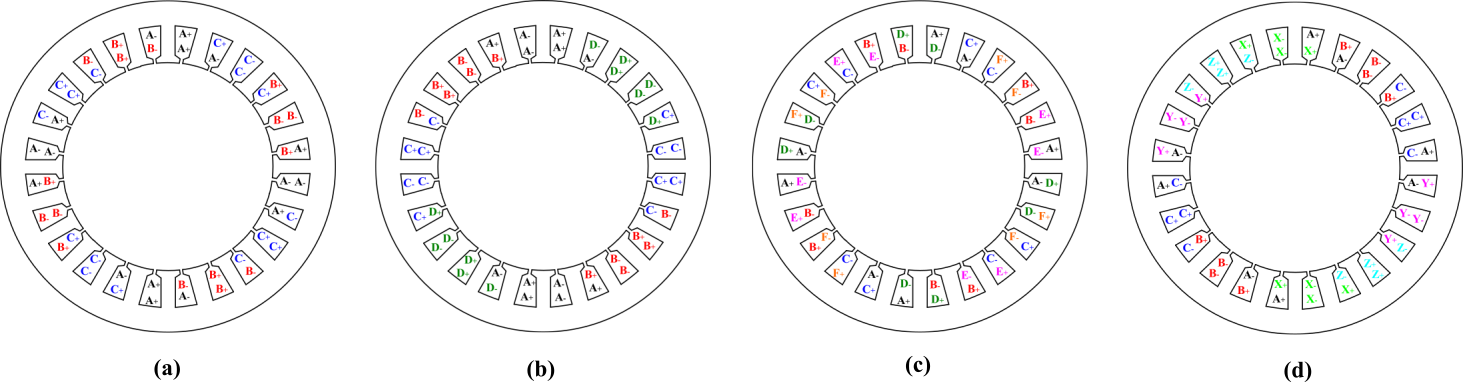
\includegraphics{windings.png}
    \caption{Winding Diagrams: (a) Three-Phase Four Modules (b) Four-Phase Two Modules (c)Symmetric Six-Phase Two Modules (d) Asymmetric Six-Phase Two Modules  }
    \label{fig:winding}
\end{figure}

\begin{comment}
\begin{table*}[ht!]
 \caption{Distribution Factors of Different Topologies for nth Harmonic Order }
\label{kd}
\begin{tabularx}{\textwidth}{@{}l*{10}{C}c@{}}
\toprule
Topology/Harmonic Order      & 1st  & 3rd & 5th & 7th & 9th & 11th & 13th \\ 
\midrule
3-Phase    & 915    & 4    & 17   & 19  & 3    & 1   & 0\%  \\ 
4-Phase    & 8      & 934  & 3    & 4   & 0    & 0   & 3\%  \\ 
Symmetric 6-Phase  & 60    & 1  & 813  & 37  & 19   & 23  & 30\%  \\ 
Asymmetric 6-Phase  & 18  & 1   & 34   & 746 & 25   & 113 & 37\%  \\

\bottomrule
\end{tabularx}
\end{table*}
\end{comment}

\section{\normalsize\textbf{Comparison of Different Topologies}}
Redundancy yüzdesi, normal operation, one phase open fault durumunda olacaklar, ilk IMMD topolojisiyle kıyaslanması, fault durumunda akımların, torque ripple ve average torque'un değişimi belirtilip karşılaştırılacak. Tablolanabilir. Akım vs gibi şeylerin simülasyonu genel olarak Simulink üzerinden yürüyecek. Tork için FEA karşılaştırması da eklenecek. Fault durumunda düzgün operate ettirmek için faz açısı kaydırma mevzularına girilecek. Genel olarak karşılaştırma bu değşik modül ve faz sayılı topolojilerin redundancy karşılaştırması üzerinden yürüyecek. 

\section{\normalsize\textbf{Conclusions}}
Toparlama. Ne yapmıştık bugün. Ne kattık biz bu çalışmayla. Experimental sonuç verecek miyiz full paperda, neleri ekleriz full papera onları yazarız.

\section{\normalsize\textbf{Future Work for Full Paper Submission}}
Bunu da ayrı başlık olarak yazalım mı? Yoksa conclusionda mı yazalım?

\AtNextBibliography{\tiny}
\printbibliography

\end{document}
